\section{Modelo Relacional}

El Modelo Relacional fue construido a partir del Modelo Entidad–Relación, transformando cada entidad en tablas y definiendo las relaciones mediante llaves primarias y llaves foráneas.

La estructura resultante se encuentra normalizada hasta la Tercera Forma Normal (3FN), reduciendo la redundancia de datos y garantizando la integridad referencial dentro del sistema.

Para facilitar la organización de la información, la base de datos fue dividida en distintos esquemas que agrupan tablas con funciones similares, tales como \texttt{catalogo}, \texttt{usuarios}, \texttt{movilidad}, \texttt{personal}, \texttt{incidentes} y \texttt{reportes}.

La Figura~\ref{fig:modelo_relacional} muestra la estructura lógica completa de la base de datos, incluyendo las tablas, atributos, llaves primarias, llaves foráneas y relaciones existentes entre los diferentes componentes del sistema.

\begin{figure}[H]
	\centering
	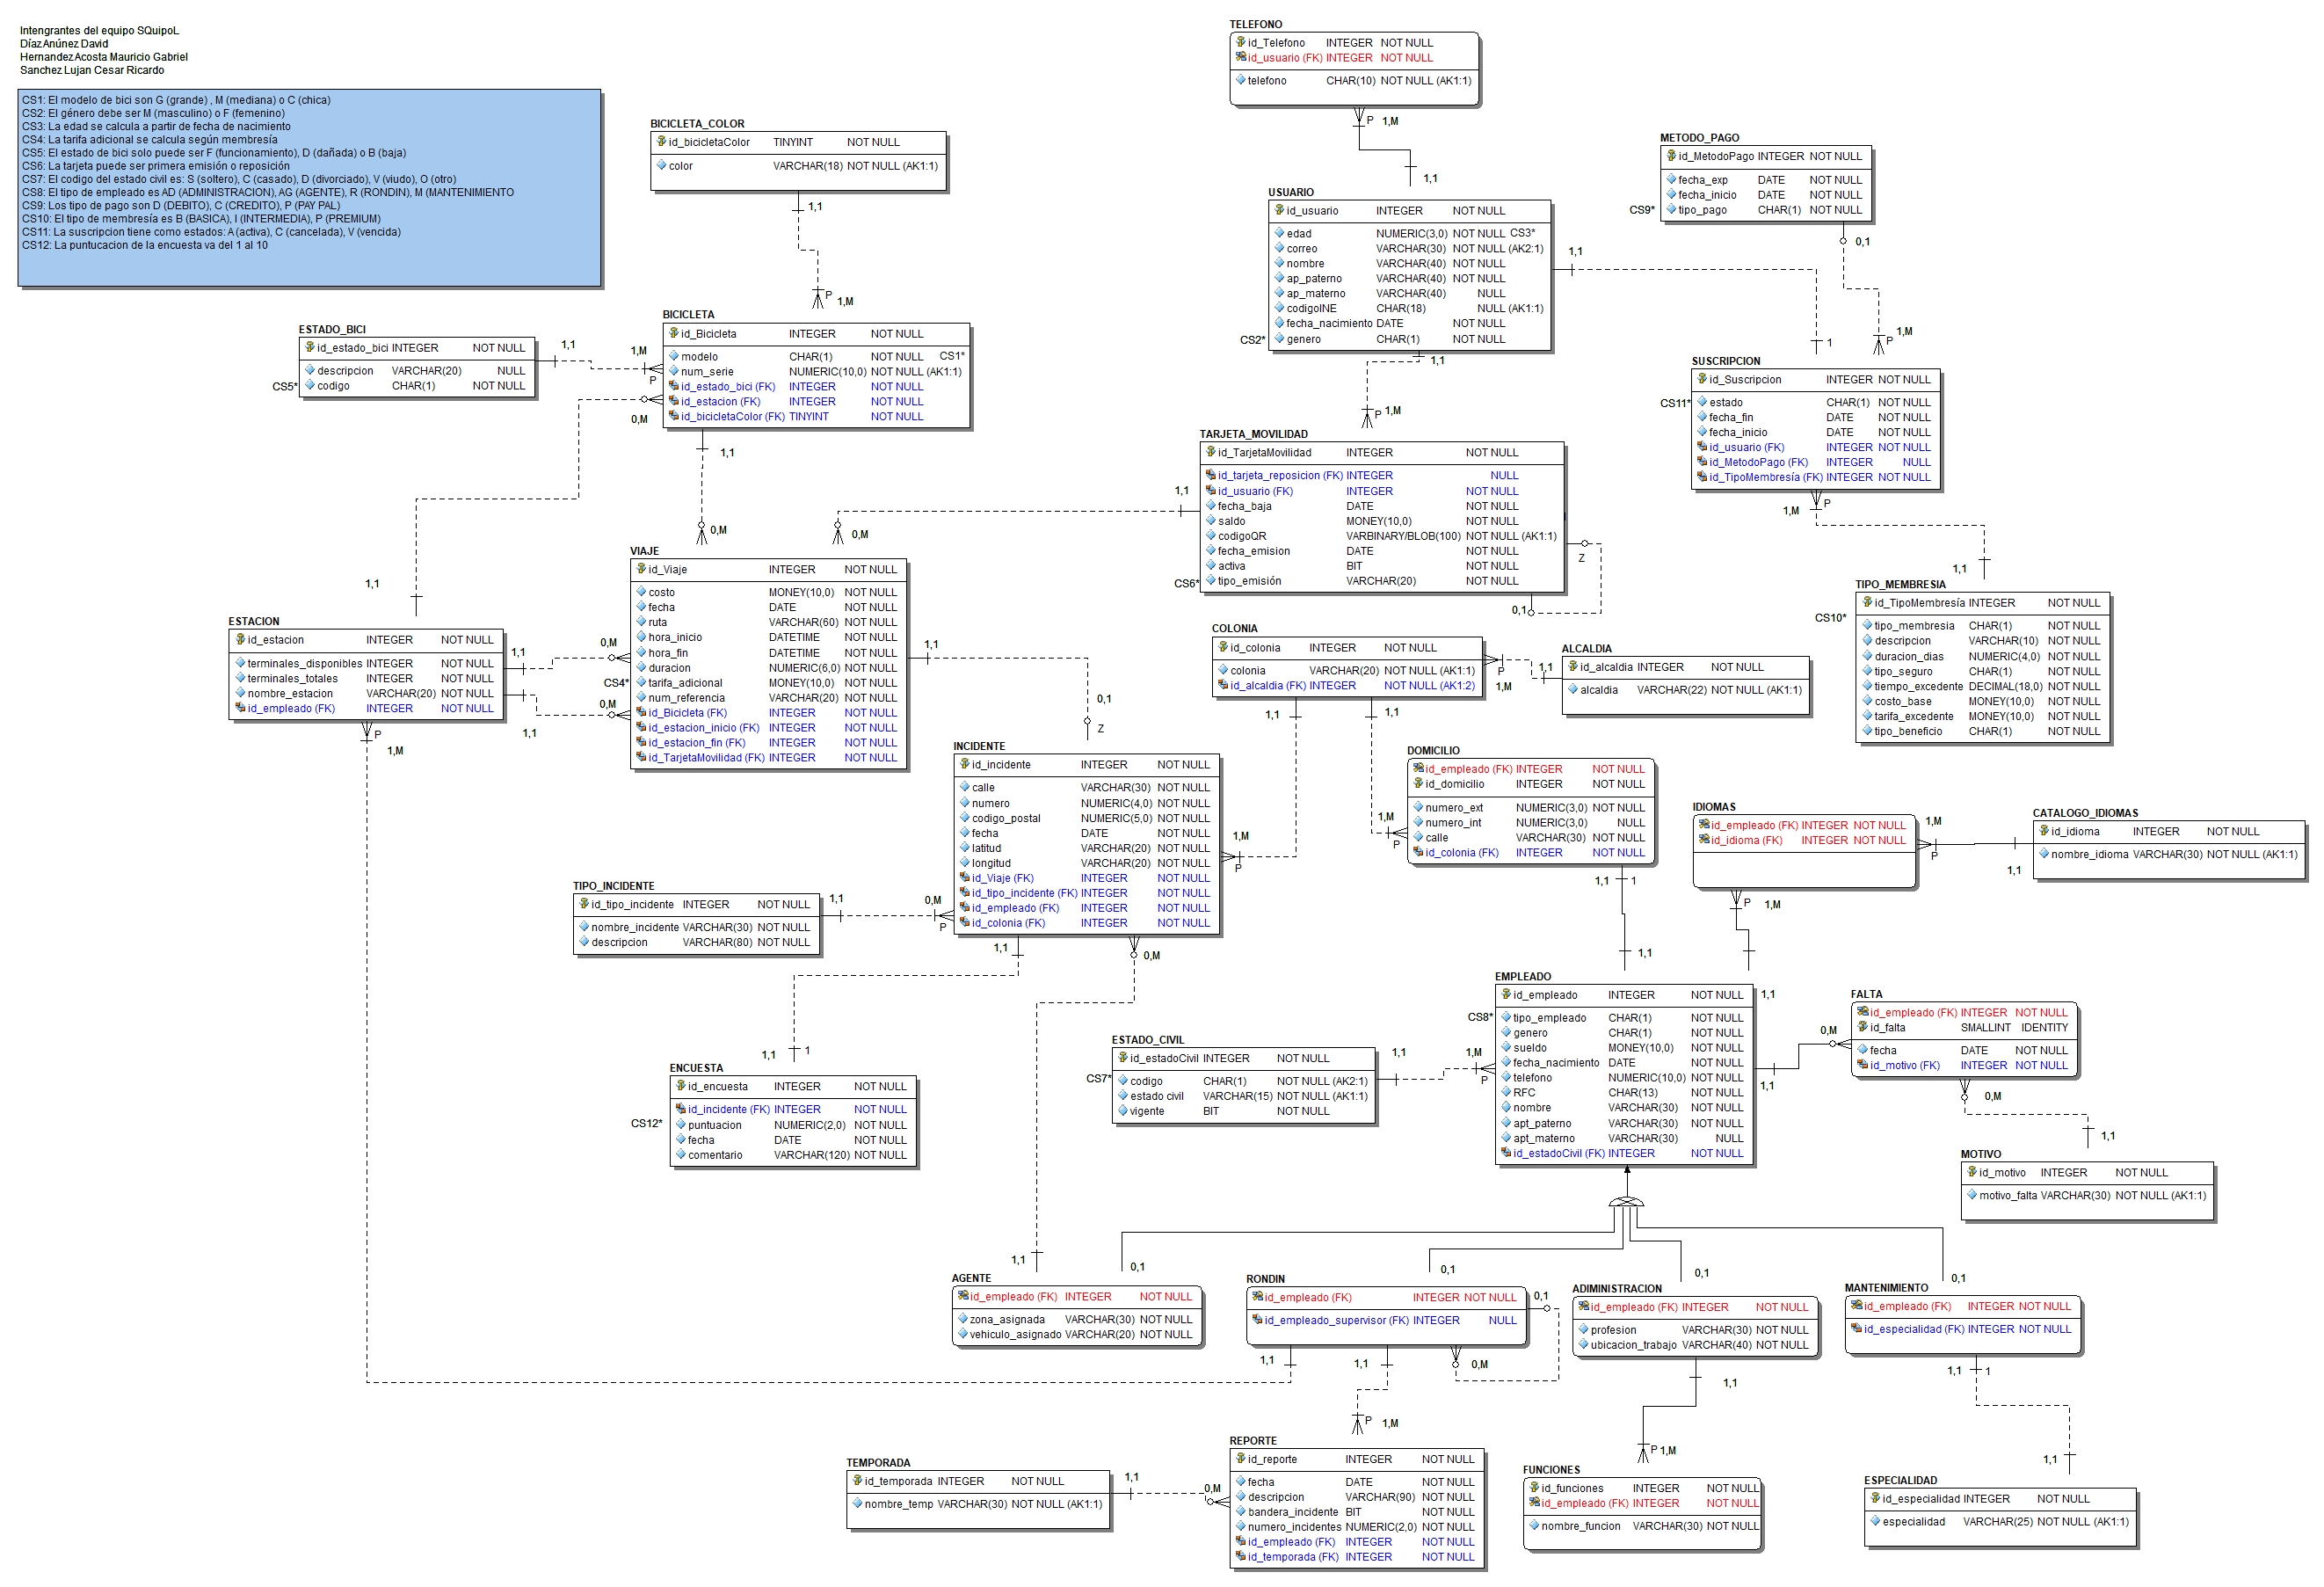
\includegraphics[width=0.9\textwidth]{figures/mr.jpg}
	\caption{Modelo Relacional del sistema ECOBICI}
	\label{fig:modelo_relacional}
\end{figure}
